\chapter{Geometría del universo en expansión}

El tema es el universo en expansión y su geometría. El objetivo es describir qué significa que el espacio se expanda antes de preguntar qué impulsa la expansión. La cosmología newtoniana \(F=ma\) se aborda más adelante, y solo después se integran la geometría y la dinámica en el marco completo de Friedmann--Robertson--Walker.

\section{Coordenadas comóviles en una línea en expansión}

Empecemos por el ejemplo más sencillo posible: el espacio unidimensional, no el espacio-tiempo. Imaginemos una línea infinita con galaxias igualmente espaciadas. La coordenada \(x\) todavía no mide una distancia física: identifica las galaxias. Podemos pensar en \(x\) como el nombre de una galaxia; ese nombre permanece asociado a ella aunque todo el conjunto se estire o se contraiga.

Sea \(a\) la distancia física entre la galaxia llamada \(x=0\) y la llamada \(x=1\). Entonces, la distancia física entre dos galaxias cualesquiera es
\begin{equation}
d=a\,\Delta x.
\end{equation}
La diferencia de coordenadas \(\Delta x\) es solo la diferencia entre sus etiquetas. El factor \(a\) convierte esa diferencia entre etiquetas en una distancia real, medida con reglas.

Imaginemos ahora que la línea es un hilo elástico que se estira. Las etiquetas permanecen asociadas a las galaxias, pero la distancia entre galaxias vecinas cambia con el tiempo. La misma relación pasa a ser
\begin{equation}
d(t)=a(t)\,\Delta x.
\end{equation}
En esta etapa, homogeneidad significa simplemente que las galaxias vecinas están igualmente espaciadas en todas partes, aunque esa separación común pueda variar con el tiempo.

\section{La ley de Hubble y la ausencia de un centro}

Para hallar la velocidad relativa de dos galaxias fijas, mantengamos fijo el par, de modo que \(\Delta x\) no cambie con el tiempo. Al derivar, obtenemos
\begin{align}
\dot d &= \dot a\,\Delta x \\
       &= \frac{\dot a}{a}\,a\,\Delta x \\
       &= \frac{\dot a}{a}\,d.
\end{align}
Si definimos
\begin{equation}
H(t)\equiv \frac{\dot a}{a},
\end{equation}
entonces
\begin{equation}
\dot d = H(t)\,d.
\end{equation}
Esta es la ley de Hubble.

La expresión histórica ``constante de Hubble'' induce a error. La cantidad es constante en el espacio, no en el tiempo. En un momento dado es la misma para todas las galaxias, pero, en general, cambia a medida que evoluciona el universo. Es más apropiado considerarla como el parámetro de Hubble.

La ley indica que las galaxias más distantes se alejan más deprisa. No señala ningún centro. Nada en el argumento privilegia \(x=0\) ni ningún otro punto. Todos los observadores ven la misma regla. Por tanto, en este modelo, el universo en expansión no es una explosión que parte de un lugar privilegiado.

El corrimiento al rojo aparece de inmediato. Si dos galaxias intercambian señales luminosas mientras se alejan una de otra, la luz recibida se desplaza hacia el rojo. Cuanto mayor es la velocidad de recesión, mayor es el corrimiento al rojo. Por tanto, las líneas espectrales nos informan sobre las velocidades de recesión. Las distancias son más difíciles de medir, y las primeras estimaciones de Hubble eran aproximadas. Su primer gráfico no era una recta perfecta, sino un conjunto disperso de puntos con grandes incertidumbres. Aun así, el principio geométrico resistió el ruido: la velocidad de recesión es proporcional a la distancia.

\begin{classroomqa}\audiencequestion{Si las galaxias están lo bastante alejadas, ¿la ley de Hubble hace que se muevan más rápido que la luz?}\lecturetimestamp{00:20:23}\lecturerresponse{Sí, en este sentido de recesión, así es. Lo que dices es correcto. Sin duda volveremos a esto. Es una de las cosas más importantes.}\end{classroomqa}

\section{Dimensiones superiores, isotropía y evolución temporal de \(a(t)\)}

Nada esencial cambia al añadir más dimensiones espaciales. En dos dimensiones, imaginemos una cuadrícula de galaxias etiquetadas por \((x,y)\), y en tres dimensiones, por \((x,y,z)\). Las coordenadas vuelven a ser etiquetas comóviles: acompañan a las galaxias en vez de medir directamente la distancia física.

¿Por qué debería ser igual la separación en la dirección \(x\) que en la dirección \(y\)? La respuesta es observacional. Si las galaxias estuvieran sistemáticamente más agrupadas en una dirección que en otra, el cielo se vería distinto según la dirección. A escalas suficientemente grandes, no es así. Esa uniformidad entre direcciones es la isotropía.

En dos dimensiones, la distancia entre dos galaxias es
\begin{equation}
d=a\sqrt{(\Delta x)^2+(\Delta y)^2},
\end{equation}
y en tres dimensiones,
\begin{equation}
d=a\sqrt{(\Delta x)^2+(\Delta y)^2+(\Delta z)^2}.
\end{equation}
Para un par fijo de galaxias, las diferencias de coordenadas permanecen constantes, así que al derivar de nuevo obtenemos
\begin{equation}
\dot d=\frac{\dot a}{a}\,d.
\end{equation}
La ley de Hubble no cambia.

Homogeneidad significa que las propiedades son iguales de un lugar a otro. Isotropía significa que son iguales en todas las direcciones. Ninguna de las dos se cumple exactamente a escalas pequeñas. No es lo mismo mirar a través de la Vía Láctea que mirar perpendicularmente a su plano, y las galaxias individuales no están distribuidas uniformemente a distancias cortas. Pero, al promediar sobre muchas galaxias, el universo a gran escala parece aproximadamente igual en todas partes y en todas las direcciones.

\begin{classroomqa}\audiencequestion{Si la velocidad es proporcional a la distancia y esta aumenta, ¿significa eso que un par fijo de galaxias debe acelerarse al alejarse una de otra?}\lecturetimestamp{00:40:22}\lecturerresponse{No. La ley de Hubble dice que, en un momento dado, la velocidad de recesión es proporcional a la distancia. Por sí sola, no indica si la velocidad de un par fijo aumenta o disminuye con el tiempo. Eso depende de la evolución temporal detallada de \(a(t)\). Si \(a(t)\propto t\), las galaxias vecinas se separan a velocidad constante. Si \(a(t)\propto t^2\), la velocidad de recesión de un par fijo aumenta con el tiempo. Si \(a(t)\propto \log t\), disminuye con el tiempo. La ley \(\dot d=(\dot a/a)d\) siempre se cumple como función de la distancia, pero la aceleración y la desaceleración son cuestiones distintas.}\end{classroomqa}

Durante mucho tiempo, los cosmólogos esperaron que el universo se estuviera desacelerando, ya que la gravedad debería frenar una expansión inicial del mismo modo que frena un objeto lanzado hacia arriba. Aquí solo nos interesa señalar que la ley de Hubble, por sí sola, no determina el comportamiento de \(\dot a\) ni de \(\ddot a\).

\begin{classroomqa}\audiencequestion{¿Cómo se fija el valor inicial del factor de escala \(a\)?}\lecturetimestamp{00:46:18}\lecturerresponse{Su normalización global es arbitraria. Lo que tiene importancia física no es el valor numérico de \(a\) por sí solo, sino cómo cambia. Si se define otro factor de escala \(b=3a\), entonces \(\dot b/b=\dot a/a\). Reescalar \(a\) por una constante cambia las convenciones o las unidades, pero no el parámetro de Hubble.}\end{classroomqa}

\section{De la métrica espacial a la métrica del espacio-tiempo}

Reemplacemos ahora \(\Delta x\) por \(dx\). La distancia física entre puntos vecinos es
\begin{equation}
ds=a\,dx,
\end{equation}
por lo que
\begin{equation}
ds^2=a^2\,dx^2.
\end{equation}
Esta es la métrica espacial en una dimensión. El coeficiente de \(dx^2\) es
\begin{equation}
g_{xx}=a^2.
\end{equation}
Así, podemos describir un universo en expansión diciendo que la parte espacial de la métrica depende del tiempo.

Para pasar del espacio al espacio-tiempo, usamos el intervalo relativista. En una dimensión espacial,
\begin{equation}
d\tau^2=dt^2-a^2(t)\,dx^2.
\end{equation}
Para un observador comóvil, \(dx=0\), así que \(d\tau=dt\). El tiempo cósmico ordinario es el tiempo propio medido por relojes que se mueven junto con las galaxias.

El dibujo de la pizarra resulta útil aquí porque reúne las líneas de universo comóviles, el elemento de línea y la notación de la métrica.
\begin{figure}[H]\centering
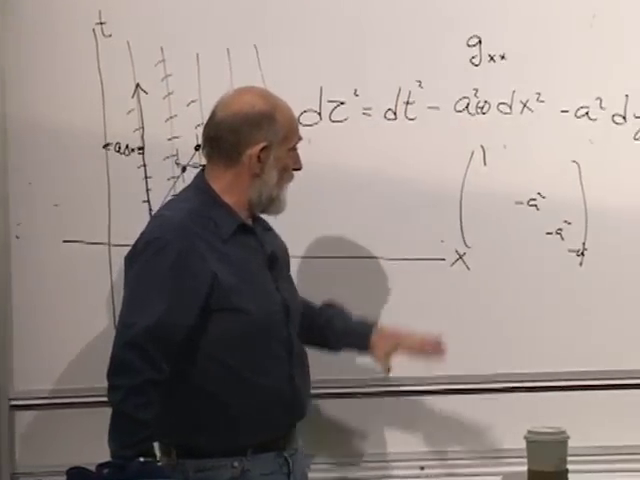
\includegraphics[width=0.82\textwidth]{lecture_01_figure_02.png}\caption{Líneas de universo comóviles en un universo unidimensional en expansión, junto con el intervalo de espacio-tiempo correspondiente.}\end{figure}

En tres dimensiones espaciales, el mismo esquema da la extensión, con las debidas precauciones\footnote{La pizarra está parcialmente oculta alrededor de 00:56:38--00:58:51. Esta forma tridimensional recoge la extensión oral de una a tres dimensiones espaciales, junto con el patrón diagonal visible en la pizarra.}
\begin{equation}
d\tau^2=dt^2-a^2(t)\bigl(dx^2+dy^2+dz^2\bigr),
\end{equation}
con métrica diagonal
\begin{equation}
g_{\mu\nu}=\mathrm{diag}\bigl(1,-a^2,-a^2,-a^2\bigr).
\end{equation}
Los términos no diagonales se anulan:
\begin{equation}
g_{tx}=g_{ty}=g_{tz}=0.
\end{equation}

La homogeneidad significa que los coeficientes de la métrica pueden depender del tiempo, pero no de la posición espacial. La isotropía significa que las tres direcciones espaciales intervienen del mismo modo.

\begin{classroomqa}\audiencequestion{¿No se supone que debemos interpretar \(dx\) como una distancia?}\lecturetimestamp{01:01:18}\lecturerresponse{No. \(dx\) no es la distancia. \(a\,dx\) es la distancia. \(dx\) es solo un intervalo entre etiquetas. Una forma útil de entenderlo es imaginar que, en cierto momento, alguien traza una cuadrícula de coordenadas a través de las galaxias y luego exige que la cuadrícula las siga. La separación entre coordenadas permanece fija por construcción, mientras que la distancia física cambia. Se podrían incluir las unidades de distancia en \(x\) en vez de en \(a\); eso es una convención. Lo que importa es el producto \(a\,dx\).}\end{classroomqa}

\begin{classroomqa}\audiencequestion{El coeficiente métrico de \(dt^2\) es igual a \(1\). ¿Eso también es solo una convención?}\lecturetimestamp{01:03:24}\lecturerresponse{Sí. Eso, por sí solo, no tiene contenido físico. Si el coeficiente dependiera solo del tiempo, se podría cambiar la variable temporal para que pasara a ser simplemente \(dt^2\). Del mismo modo, se pueden elegir unidades en las que \(c=1\). Lo que aquí no es una convención es que el coeficiente no dependa de la posición, aunque sí pueda depender del tiempo.}\end{classroomqa}

\begin{classroomqa}\audiencequestion{Si se introduce esto en las ecuaciones de campo de Einstein, ¿qué se obtiene para el tensor de energía-momento?}\lecturetimestamp{01:05:59}\lecturerresponse{Ese es el tipo de pregunta que viene a continuación, pero pertenece a la dinámica, no al tema que estamos tratando ahora. Se puede introducir esta métrica en las ecuaciones de Einstein y preguntar qué distribución de energía-momento haría que fuera una solución. Eso es muy importante, pero por el momento nos ocupamos de la geometría, no de la dinámica.}\end{classroomqa}

\section{Lo que oculta el horizonte}

El universo a gran escala se considera homogéneo e isótropo solo como aproximación. Desde luego, no es homogéneo a la escala de las estrellas, los planetas ni siquiera las galaxias individuales. Tampoco es exactamente isótropo en todas las observaciones locales.

Un campo de cultivo ilustra bien la dependencia de la escala. A cierta escala parece regular; a una escala mucho menor, evidentemente no lo es; y a una escala mayor que el campo entero, deja de parecer homogéneo otra vez. En cosmología ocurre lo mismo. Tras promediar sobre muchas galaxias, la distribución a gran escala parece aproximadamente uniforme. A escalas suficientemente pequeñas, no lo es.

El universo es más grande que la parte que podemos ver, y más grande que la parte que podremos ver jamás. En las escalas que realmente podemos explorar, es isótropo y homogéneo, salvo por variaciones locales. Más allá de eso, no hay ninguna garantía observacional directa.

\begin{classroomqa}\audiencequestion{Dijo que nunca llegaremos a saberlo directamente. ¿Eso implica que quizá haya una forma indirecta de averiguarlo?}\lecturetimestamp{01:10:34}\lecturerresponse{Quizá. Hoy en día, la mayoría piensa que, a escalas suficientemente grandes, el universo no es homogéneo, y yo apuesto por lo mismo. Pero es una apuesta que nunca podré ganar ni perder, porque, por razones fundamentales, no podremos ver mucho más allá de lo que vemos ahora. Eso se debe a la existencia de un horizonte.}\end{classroomqa}

\begin{classroomqa}\audiencequestion{¿No se podría usar la gravedad para buscar masas más allá de lo que podemos ver?}\lecturetimestamp{01:11:53}\lecturerresponse{No. Una masa distante puede simplemente hacernos caer en caída libre. Estamos en una habitación cerrada, dentro del campo gravitatorio del Sol y orbitándolo, pero, si no podemos mirar al exterior, no hay una manera fácil de saber que el Sol está ahí. Solo las fuerzas de marea lo revelarían y, si la fuente estuviera lo bastante lejos, esos efectos de marea podrían ser demasiado pequeños para detectarlos.}\end{classroomqa}

Por tanto, el horizonte es una barrera definitiva para el conocimiento directo. Incluso afirma, con prácticamente total certeza, que el volumen del universo es al menos mil veces mayor que el de la región que jamás podremos ver, y deja para más adelante la explicación de esa afirmación.

\section{Finito y sin frontera}

Pasemos ahora a las geometrías cerradas. La línea infinita es abierta e ilimitada. Un segmento de recta es acotado, en el sentido de que tiene una extensión finita. Acotado no significa que tenga una frontera, sino que su extensión es finita.

Un cubo con paredes no sirve. Viola la homogeneidad, porque alguien cerca de una pared no es equivalente a alguien lejos de ella, y viola la isotropía, porque incluso quien está en el centro ve cosas distintas en distintas direcciones.

El interior de un círculo o de una esfera tampoco sirve. Alguien en el centro ve lo mismo en todas las direcciones, pero esa simetría solo corresponde a un punto especial. Si se aleja del centro, la pared está cerca en una dirección y lejos en otra. Por tanto, para observadores genéricos, el espacio no es ni homogéneo ni isótropo.

La hipótesis de trabajo a escalas muy grandes es que el universo es homogéneo e isótropo. Este es el principio cosmológico. Es útil, pero nada impide que se revise.

\begin{classroomqa}\audiencequestion{¿La isotropía en todas partes implica homogeneidad?}\lecturetimestamp{01:18:57}\lecturerresponse{Sí. Si todos los observadores ven lo mismo en todas las direcciones, eso implica homogeneidad. Pero la implicación inversa no se cumple. La homogeneidad por sí sola no implica isotropía. Un universo puede ser homogéneo y, aun así, tener una dirección privilegiada; por ejemplo, si estuviera lleno de flechas que apuntaran todas en la misma dirección.}\end{classroomqa}

El modelo acotado adecuado es la superficie de una esfera sin rasgos distintivos. Una criatura bidimensional confinada a esa superficie encuentra cada lugar localmente igual a cualquier otro y cada dirección igual a cualquier otra, aunque el mundo sea finito. Eso es ser finito y carecer de frontera.

\section{Un universo unidimensional cerrado en forma de círculo}

Para simplificar el álgebra, reduzcamos el ejemplo de la esfera a una dimensión espacial: la vida en un círculo. En una dimensión, isotropía significa que izquierda y derecha son equivalentes. Un círculo tiene exactamente esa propiedad. Elijamos un punto y llamémoslo \(\theta=0\). A todos los demás puntos se les asigna una coordenada angular \(\theta\), medida en radianes. Un punto justo a un lado del origen puede describirse con un ángulo negativo pequeño o con uno apenas menor que \(2\pi\). Esa periodicidad forma parte de la geometría.

Los habitantes del círculo tienen acceso a la circunferencia, no a un radio ni a un centro externos. Pueden medir la distancia total alrededor recorriendo el círculo hasta regresar al mismo punto. Si se dibuja el círculo en un plano que lo contiene, también se puede introducir una cantidad análoga al radio, pero eso pertenece a la representación mediante una inmersión, no a la geometría intrínseca que ellos miden.

El dibujo de la pizarra es útil aquí porque muestra en un mismo esquema las etiquetas angulares y la circunferencia total.
\begin{figure}[H]\centering
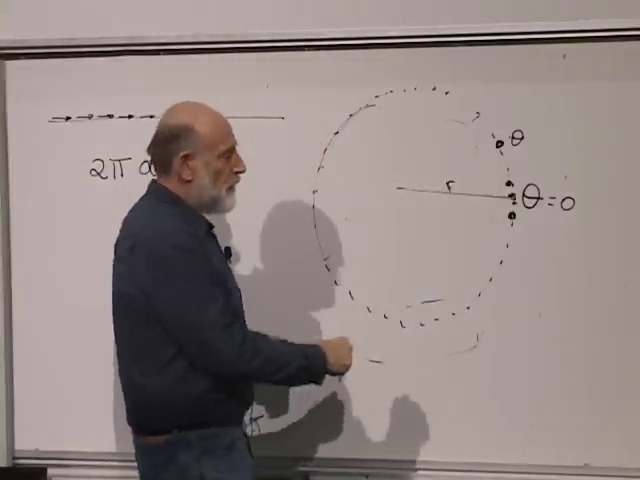
\includegraphics[width=0.82\textwidth]{lecture_01_figure_03.png}\caption{Descripción angular de un universo unidimensional cerrado, con circunferencia total \(2\pi a\).}\end{figure}

Una convención práctica es\footnote{En torno a 01:26:40--01:29:20, la notación cambia brevemente entre tomar la circunferencia completa como factor de escala y escribirla como \(2\pi a\). Aquí se usa la convención posterior, porque es la que se incorpora a la fórmula de longitud de arco.}
\begin{equation}
L=2\pi a,
\end{equation}
donde \(L\) es la circunferencia total.

Para una pequeña separación angular \(\Delta\theta\), la distancia física es
\begin{equation}
d=a\,\Delta\theta.
\end{equation}
Al pasar a diferenciales, se obtiene
\begin{equation}
ds=a\,d\theta,
\end{equation}
y, por tanto,
\begin{equation}
ds^2=a^2\,d\theta^2.
\end{equation}
Esta es la métrica local del círculo.

Si \(a\) depende del tiempo, el universo unidimensional cerrado se expande o se contrae. Para un par fijo de galaxias,
\begin{equation}
d(t)=a(t)\,\Delta\theta,
\end{equation}
por lo que
\begin{equation}
\dot d=\dot a\,\Delta\theta
      =\frac{\dot a}{a}\,d.
\end{equation}
La ley de Hubble también se cumple aquí, al menos para pares que no estén tan alejados que resulte ambiguo cuál de los dos caminos alrededor del círculo se toma.

La métrica del espacio-tiempo pasa a ser
\begin{equation}
d\tau^2=dt^2-a^2(t)\,d\theta^2.
\end{equation}
Si \(a\) es constante, la representación del espacio-tiempo es un cilindro. Si \(a\propto t\), es un cono. Si \(a(t)\) cambia de manera más irregular, la representación adquiere forma de vaso.

Si seguimos el dibujo hacia atrás en el tiempo, las galaxias se acercan cada vez más. Si hubiera \(360\) galaxias alrededor del círculo, estarían bien separadas en épocas tardías, muy juntas en épocas anteriores y aún más juntas antes. Al final dejarían de ser galaxias separadas y, en épocas todavía anteriores, ni siquiera serían átomos separados. Pero sigue sin haber ningún punto especial en el espacio.

Esta es la respuesta más clara, dentro del modelo, a la pregunta de dónde ocurrió el Big Bang. Cuando \(a(t)\to 0\), todas las separaciones \(a(t)\,\Delta\theta\) se anulan. El universo entero se contrae en todas partes a la vez. Las galaxias no salen disparadas desde un lugar privilegiado hacia un espacio exterior. Lo que cambia de escala es la propia geometría. En ese sentido, la respuesta es: en todas partes.

\begin{classroomqa}\audiencequestion{Dijo que el espacio-tiempo está curvado. ¿Estaría curvado si tuviera forma de cilindro?}\lecturetimestamp{01:38:04}\lecturerresponse{No. Si tuviera forma de cilindro, no estaría curvado. Ese es el caso en que \(a\) es constante en el tiempo. Solo parece curvado porque se dibuja en un espacio de más dimensiones. Si se corta y se abre, se puede extender plano sin estirarlo.}\end{classroomqa}

A partir de ahí, la discusión pasa al cono. Si \(a\propto t\), la representación del espacio-tiempo es un cono. Salvo en su vértice, el cono también es plano en el mismo sentido intrínseco: se puede abrir para formar un plano. El vértice es distinto. Es una singularidad cónica.

El siguiente paso es estudiar la geometría del universo esférico y, después, la dinámica que determina cómo \(a(t)\) crece o se contrae.
